%        1         2         3         4         5         6         7         8         9         0         1         2
%23456789012345678901234567890123456789012345678901234567890123456789012345678901234567890123456789012345678901234567890
\documentclass[12pt]{MIA-USA}

\usepackage{layout}
\usepackage{subcaption}
\usepackage{paralist}
\usepackage{breakcites}

\usepackage[pagebackref=true,breaklinks=true]{hyperref}
\hypersetup{
	pdftitle={Documento de trabajo Final}, 
	pdfauthor={MIA-D.Martinez}, 
	pdfsubject={}, 
	pdfcreator={DarMart with Latex}, 
	colorlinks=true,
	linkcolor=GrisUno,
	citecolor=AzulInstitucional,
	filecolor=AzulClaro,
	urlcolor=AzulInstitucional,
	linktoc=all
}

\graphicspath{{Images/}}


\title{T\'itulo del proyecto}
\author{Nombres y apellidos Estudiante}
\documenttype{Docuemnto Final}

\advisor{Nombres y apellidos Asesor}

% Si hay un coasesor 
% \coadvisor{Nombres y apellidos Co-Asesor}


% Aqui comienza el documento
% - -- --- ----- ------- ------- ----- --- -- -
\begin{document}
    % \layout{}
	
	\maketitle
	% Incluye la pagina de acptación (Opcional)
	% Página de aceptación. Contiene las firmas del presidente o director y de los jurados que participan en la revisión, sustentación y aprobación del trabajo. Adicionalmente, incluye la ciudad y la fecha de entrega (día, mes, año), conservando los márgenes establecidos

{\hfill
    \begin{minipage}{0.5\textwidth}
        \centering
        
        Nota de aceptaci\'on:\\
        \vspace*{0.8cm}
        
        \hrulefill\\[0.2cm]
        \hrulefill\\[0.2cm]
        \hrulefill\\[0.2cm]
        \hrulefill\\[0.2cm]
        \hrulefill\\[0.2cm]
        \hrulefill\\
        \vspace*{4cm}
        
        \hrulefill\\
        Firma del presidente del jurado\\
        \vspace*{2.5cm}
        
        \hrulefill\\
        Firma del jurado\\
        \vspace*{2.5cm}
        
        \hrulefill\\
        Firma del jurado\\
        \vspace*{2.5cm}
    
    \end{minipage}
}
\newpage
	% Incluye la dedicatoria (Opcional)
	% Dedicatoria - Borrador
\begin{dedication}

A mi familia, por su apoyo constante y por creer en este proyecto desde sus primeras ideas. A mis amigos y colegas, por sus consejos y paciencia en las largas jornadas de trabajo.

\end{dedication}

	% Incluye los agradecimientos (Opcional)
	% Agradecimientos - Borrador
\begin{acknowledgements}

Quiero expresar mi sincero agradecimiento al director de proyecto, Dr. [Nombre del Director], por su orientación experta, sus observaciones críticas y su compromiso con la excelencia académica. Agradezco también al equipo de desarrollo y a los colaboradores de la empresa XCargo por facilitar el acceso a datos y por sus valiosas observaciones en cada iteración del prototipo.

A mi familia, por su apoyo incondicional; y a mis amigos por las charlas que ayudaron a clarificar ideas en momentos clave.

\end{acknowledgements}

	% Resumen
    % Presentación abreviada y precisa del contenido de un documento, sin agregar interpretación o crítica y se recomienda un exceda una página.
\section*{Resumen}

El resumen es una presentación abreviada y precisa del contenido de un documento, sin agregar interpretación o crítica. Para documentos extensos como informes, tesis y trabajos de grado, no debe exceder de 500 palabras, y debe ser lo suficientemente breve para que no ocupe más de una página~\cite{NTC14862008}. Se recomienda que este resumen sea anal\'{\i}tico, es decir, que sea completo, con informaci\'{o}n cuantitativa y cualitativa, generalmente incluyendo los siguientes aspectos: objetivos, dise\~{n}o, lugar y circunstancias, pacientes (u objetivo del estudio), intervenci\'{o}n, mediciones y principales resultados, y conclusiones. Al final del resumen se deben usar palabras claves tomadas del texto (m\'{\i}nimo 3 y m\'{a}ximo 10 palabras), las cuales permiten la recuperaci\'{o}n de la informaci\'{o}n.\\

\textbf{\small Palabras clave: (m\'{a}ximo 10 palabras, preferiblemente seleccionadas de las listas internacionales que permitan el indizado cruzado)}.\\

% debe incluir una lista de palabras clave 
\textbf{Palabras clave}: palabra 1, palabra 2, palabra 3, ...

% Incluir un resumen en otro idioma de preferencia inglés
\newpage
\section*{Abstract}

% debe incluir una lista de palabras clave en el otro idioma
\textbf{Keywords}: Keyword 1, Keyword 2, Keyword 3, ...
% Resumen (Abstract) - Contenido actualizado por integración de borrador
\begin{abstract}

Este trabajo presenta el dise\\~{n}o, implementaci\\'on y evaluaci\\'on de XCargo, una plataforma integral para la gesti\\'on log\\'istica de env\\'ios y liquidaci\\'on de gu\\'ias dirigida a peque\\~{n}as y medianas empresas de transporte. XCargo integra una interfaz web para operadores y conductores, un backend basado en FastAPI que centraliza la l\\'ogica de negocio y almacenamiento en Google BigQuery para registro y conciliaci\\'on de pagos.

Se propone un flujo seguro y trazable para el registro de pagos de conductores, la gesti\\'on de comprobantes digitales y la conciliaci\\'on contable. La soluci\\'on aborda problemas comunes en el sector como la falta de trazabilidad en el proceso de cobro, la dificultad para conciliar movimientos bancarios con referencias de pago, y la necesidad de reportes por carrier y por periodo.

En la implementaci\\'on se describen los m\\'odulos principales: autenticaci\\'on y control de acceso por roles y permisos, captura y validaci\\'on de comprobantes, almacenamiento y consulta anal\\'itica en BigQuery, y herramientas de supervisi\\'on y conciliaci\\'on. Se presenta una evaluaci\\'on funcional que incluye pruebas de caso real, pruebas de integridad de datos y consideraciones de seguridad y rendimiento.

Finalmente, se discuten las limitaciones del prototipo, recomendaciones para despliegue en producci\\'on y las l\\'ineas de trabajo futuro, que incluyen: mejora de la seguridad de autenticaci\\'on (rotaci\\'on de claves y refresh tokens), optimizaci\\'on de consultas en BigQuery para reducir costos, y un m\\'odulo de automatizaci\\'on de conciliaci\\'on bancaria.

\end{abstract}


	
    
    % Crea la tabla de contenidos a partir de la estructura del documento
    \tableofcontents
    % Crea la lista de figuras (Opcional)
    \listoffigures
    % Crea la lista de tablas (Opcional)
    \listoftables
    % Incluye la lista de simbolos (Opcional)
    \chapter*{Lista de s\'{\i}mbolos}
% \addcontentsline{toc}{chapter}{\numberline{}Lista de s\'{\i}mbolos}
\addcontentsline{toc}{chapter}{\hspace{1em} Lista de s\'{\i}mbolos}
Esta secci\'{o}n es opcional, dado que existen disciplinas que no manejan s\'{\i}mbolos y/o abreviaturas. A continuaci\'on se presentan algunos ejemplos tomados de la plantilla de Tesis de Maestr\'ia y doctorado de la Universidad Nacional.\\

Se incluyen s\'{\i}mbolos generales (con letras latinas y griegas), sub\'{\i}ndices, super\'{\i}ndices y abreviaturas (incluir s\'{o}lo las clases de s\'{\i}mbolos que se utilicen). Cada una de estas listas debe estar ubicada en orden alfab\'{e}tico de acuerdo con la primera letra del s\'{\i}mbolo.
\section*{S\'{\i}mbolos con letras latinas}
 \label{simbolos}
 \renewcommand{\arraystretch}{1.3}
%\begin{longtable}[l]{*{4}{>{$}l<{$}}p{9cm}}
\begin{longtable}[l]{>{$}l<{$}l>{$}l<{$}>{$}l<{$}}
%\begin{tabular}
\textbf{S\'{\i}mbolo}&\textbf{T\'{e}rmino}&\textbf{Unidad SI}&\textbf{Definici\'{o}n}\\[0.5ex]\hline
\endfirsthead%
\textbf{S\'{\i}mbolo}&\textbf{T\'{e}rmino}&\textbf{Unidad SI}&\textbf{Definici\'{o}n}\\[0.5ex]\hline
\endhead%
      A              &\'{A}rea                                   &\text{m}^{2}                         &\int\int dxdy\\%
      A_{\text{BET}} &\'{A}rea interna del s\'{o}lido                &\frac{\text{m}^{2}}{\text{g}}        &\text{ver DIN ISO 9277}\\%
      A_{\text{g}}   &\'{A}rea transversal de la fase gaseosa    &\text{m}^{2}                         &\text{Ec...}\\%
      A_{\text{s}}   &\'{A}rea transversal de la carga a granel  &\text{m}^{2}                         &\text{Ec...}\\%
      a              &Coeficiente                            &1                                    &\text{Ec...}\\%
      a              &Contenido de ceniza                    &1                                    &\frac{m_{\text{ceniza}}}{m_{\text{bm,0}}}\\%
      c              &Contenido de carbono                   &1                                    &\frac{m_{\text{C}}}{m}\\%
      c              &Longitud de la cuerda                  &\text{m}                             &\text{Figura...}\\
      c              &Concentraci\'{o}n de la cantidad de materia&\frac{\text{mol}}{\text{m}^{3}}      &\frac{n}{V}\\%
      D              &Di\'{a}metro                               &\text{m}                             &\\%
      E_{\text{A}}   &Energ\'{\i}a de activaci\'{o}n                  &\frac{\text{kJ}}{\text{mol}}         &\text{Ec....}\\%
      F              &Fracci\'{o}n de materia vol\'{a}til            &1                                    &\text{ver DIN 51720}\\%
      Fr             &N\'{u}mero de Froude                       &1                                    &\frac{\omega^{2}R}{g_{\text{0}}}\\%
      \overrightarrow{g}&Aceleraci\'{o}n de la gravedad          &\frac{\text{m}}{\text{s}^{2}}        &\frac{d^{2}\overrightarrow{r}}{dt^{2}}\\%
      H              &Entalp\'{\i}a                               &\text{J}                             &U+PV\\%
      H_{\text{o}}   &Poder calor\'{\i}fico superior              &\frac{\text{MJ}}{\text{kg}}          &\text{ver DIN 51857}\\%
      h              &Contenido de hidr\'{o}geno                 &1                                    &\frac{m_{\text{H}}}{m}\\%
      K              &Coeficiente de equilibrio              &1                                    &\text{Ec...}\\%
      L              &Longitud                               &\text{m}                             &DF\\%
      L              &Longitud del reactor                   &\text{m}                             &\text{Figura...}\\%
      m              &Masa                                   &\text{kg}                            &DF\\%
      \dot{m}        &Flujo de masa                          &\frac{\text{kg}}{\text{s}}           &\frac{m}{t}\\%
      n              &Velocidad de rotaci\'{o}n                  &\frac{\text{1}}{\text{s}}            &\frac{\omega}{2\pi}\\%
      n              &Cantidad de materia                    &\text{mol}                           &DF\\%
      P              &Presi\'{o}n                                &\text{Pa}                            &\frac{\vec{F}\cdot\vec{n}}{A}\\%
      Q              &Calor                                  &\text{kJ}                            &\text{1. $LT$}\\%
      T              &Temperatura                            &\text{K}                             &DF\\%
      t              &Tiempo                                 &\text{s}                             &DF\\%
      x_{\text{i}}   &Fracci\'{o}n de la cantidad de materia     &1                                    &\frac{n_{\text{i}}}{n}\\%
      V              &Volumen                                &\text{m}^{3}                         &\int{dr^{3}}\\%
      \vec{u}        &Velocidad                              &\frac{\text{m}}{\text{s}}            &(\frac{dr}{dt},r\frac{d\upsilon}{dt},\frac{dz}{dt})\\%
      w_{\text{i}}   &Fracci\'{o}n en masa del componente i      &1                                    &\frac{m_{\text{i}}}{m_{\text{0}}}\\%
      w_{\text{w,i}} &Contenido de humedad de la sustancia i &1                                    &\frac{m_{\text{\wasser}}}{m_{\text{i,0}}}\\%
      Z              &Factor de gases reales                 &1                                    &\frac{pv}{RT}\\%
\end{longtable}
\vspace{5ex}
\section*{S\'{\i}mbolos con letras griegas}

\begin{longtable}[l]{>{$}l<{$}l>{$}l<{$}>{$}l<{$}}
\textbf{S\'{\i}mbolo}&\textbf{T\'{e}rmino}&\textbf{Unidad SI}&\textbf{Definici\'{o}n}\\[0.5ex] \hline%
\endfirsthead%
\textbf{S\'{\i}mbolo}&\textbf{T\'{e}rmino}&\textbf{Unidad SI}&\textbf{Definici\'{o}n}\\[0.5ex] \hline%
\endhead%
\renewcommand{\arraystretch}{1.3}
 \label{simbolosg}
     \alpha_{\text{BET}}  &Factor de superficie                  &\frac{\text{m}^{2}}{\text{g}}   &(w_{\text{F,waf}})(A_{\text{BET}})\\%
     \beta_{\text{i}}     &Grado de formaci\'{o}n del componente i   &1                               &\frac{m_{\text{i}}}{m_{\text{bm,0}}}\\%
     \gamma               &Wandhaftreibwinkel (Stahlblech)       &1                               &\text{Secci\'{o}n...}\\
     \epsilon             &Porosidad de la part\'{\i}cula             &1                               &1-\frac{\rho_{\text{s}}}{\rho_{\text{w}}}\\%
     \eta                 &mittlere Bettneigungswinkel (St\"{u}rzen) &1                               &\text{Figura...}\\%
     \theta               &\'{A}ngulo de inclinaci\'{o}n de la cama      &1                               &\text{Figura...}\\
     \theta_{\text{O}}    &\'{A}ngulo superior de avalancha          &1                               &\text{Figura...}\\
     \theta_{\text{U}}    &\'{A}ngulo inferior de avalancha          &1                               &\text{Figura...}\\
     \kappa               &Velocidad de calentamientoe           &\frac{\text{K}}{\text{s}}       &\frac{dT}{dt}\\%
     \nu                  &Coeficiente estequiom\'{e}trico           &1                               &\text{ver DIN 13345}\\%
     \rho_{\text{b}}      &Densidad a granel                     &\frac{\text{kg}}{\text{m}^{3}}  &\frac{m_{\text{S}}}{V_{\text{S}}}\;(\text{Secci\'{o}n...})\\
     \rho_{\text{s}}      &Densidad aparente                     &\frac{\text{kg}}{\text{m}^{3}}  &\frac{m_{\text{F}}}{V_{\text{P}}}\;(\text{Secci\'{o}n...})\\
     \rho_{\text{w}}      &Densidad verdadera                    &\frac{\text{kg}}{\text{m}^{3}}  &\frac{m_{\text{F}}}{V_{\text{F}}}\;(\text{Secci\'{o}n...})\\
     \tau                 &Tiempo adimensional                   &1                               &\text{Ec....}\\%
     \Phi_{\text{V}}      &Flujo volum\'{e}trico                     &\frac{\text{m}^{3}}{\text{s}}   &\frac{\Delta V}{\Delta t}\\
     \omega               &Velocidad angular                     &\frac{1}{\text{s}}              &\frac{d\upsilon}{dt}\\

\end{longtable}


\section*{Sub\'{\i}ndices}
\begin{longtable}[l]{>{}l<{}l}
  \textbf{Sub\'{\i}ndice} & \textbf{T\'{e}rmino} \\[0.5ex] \hline%
  \endfirsthead%
  \textbf{Sub\'{\i}ndice} & \textbf{T\'{e}rmino} \\[0.5ex] \hline%
  \endhead%
\renewcommand{\arraystretch}{1.4}\label{simbolosg}

 bm&materia org\'{a}nica\\%
 DR&Dubinin-Radushkevich\\%
 E&Experimental\\%
 g&Fase gaseosa\\%
 k&Condensado\\%
 Ma&Macroporos\\%
 P&Part\'{\i}cula\\%
 p&Poro\\%
 p&Pirolizado\\%
 R&Reacci\'{o}n\\%
 t&Total\\%
 wf&Libre de agua\\%
 waf&Libre de agua y de ceniza\\%
 0&Estado de referencia\\%

\end{longtable}


\setlength{\extrarowheight}{0pt}


\section*{Super\'{\i}ndices}
\begin{longtable}[l]{>{}l<{}l}
  \textbf{Super\'{\i}ndice} & \textbf{T\'{e}rmino} \\[0.5ex] \hline%
  \endfirsthead%
  \textbf{Super\'{\i}ndice} & \textbf{T\'{e}rmino} \\[0.5ex] \hline%
  \endhead%
\renewcommand{\arraystretch}{1.4}\label{simbolosg}

 n &Coeficiente x\\%



\end{longtable}


\setlength{\extrarowheight}{0pt}


\section*{Abreviaturas}
\begin{longtable}[l]{>{}l<{}l}
  \textbf{Abreviatura} & \textbf{T\'{e}rmino} \\[0.5ex] \hline%
  \endfirsthead%
  \textbf{Abreviatura} & \textbf{T\'{e}rmino} \\[0.5ex] \hline%
  \endhead%
\renewcommand{\arraystretch}{1.4}\label{simbolosg}
 1.$LT$&Primera ley de la termodin\'{a}mica\\%
 $DF$    &Dimensi\'{o}n fundamental\\%
 $RFF$   &Racimos de fruta fresca\\%

\end{longtable}


\setlength{\extrarowheight}{0pt}
    % Glosario (Opcional)
    % Lista alfabética de términos y sus definiciones o explicaciones necesarios para la comprensión del documento. La existencia de un glosario no justifica la omisión de una explicación en el texto la primera vez que aparece un término. El título glosario se escribe en mayúscula sostenida, centrado, a 3 cm del borde superior de la hoja.  El primer término aparece a dos interlíneas del título glosario, contra el margen izquierdo. Los términos se escriben con mayúscula sostenida seguidos de dos puntos y en orden alfabético. La definición correspondiente se coloca después de los dos puntos, se deja un espacio y se inicia con minúscula. Si ocupa más de un renglón, el segundo y los subsiguientes comienzan contra el margen izquierdo. Entre término y término se deja una interlínea. Su uso es opcional

\chapter*{Glosario}

Lista alfabética de términos y sus definiciones o explicaciones necesarios para la comprensión del documento. La existencia de un glosario no justifica la omisión de una explicación en el texto la primera vez que aparece un término. El título glosario se escribe en mayúscula sostenida, centrado, a 3 cm del borde superior de la hoja.  El primer término aparece a dos interlíneas del título glosario, contra el margen izquierdo. Los términos se escriben con mayúscula sostenida seguidos de dos puntos y en orden alfabético. La definición correspondiente se coloca después de los dos puntos, se deja un espacio y se inicia con minúscula. Si ocupa más de un renglón, el segundo y los subsiguientes comienzan contra el margen izquierdo. Entre término y término se deja una interlínea. Su uso es opcional~\cite{NTC14862008}
    
    
    % A partir de este punto se crea la estructura del documento con un archivo por capitulo conservando la siguiente jerarquía
    % chapter (Capitulo)
    %   - section (sección)
    %       - subsection (subsección)
    %           - subsubsection (subsubsección)
    
    % Introduction
    \chapter{Introducci\'on}
    % Introducción - Borrador
\chapter{Introducción}

En los últimos años, el sector logístico ha experimentado una aceleración en la adopción de soluciones digitales para optimizar la operación de envíos y la gestión administrativa asociada. Aun así, muchas empresas medianas y pequeñas enfrentan desafíos para mantener trazabilidad en el proceso de pago a conductores, conciliación contable y gestión de comprobantes digitales.

Este proyecto propone XCargo: una plataforma orientada a mejorar la trazabilidad y eficiencia de los procesos de liquidación y conciliación de pagos para empresas de transporte. El prototipo contempla:

- Un sistema de autenticación basado en roles (admin, master, supervisor, operador, conductor) que controla el acceso a funciones críticas.
- Un proceso para la recepción y almacenamiento seguro de comprobantes digitales, con vínculos a registros de pago en BigQuery.
- Módulos para conciliación contable que unifican movimientos bancarios y pagos reportados por conductores.

Objetivo general, objetivos específicos y la estructura del documento se presentan en la siguiente sección. Se describe además el alcance del prototipo y las limitaciones que guían las recomendaciones de trabajo futuro.


    % Problema de investigacion
    \chapter{Problema de investigaci\'on}
    % Planteamiento del problema - Borrador profesional
\section{Planteamiento del problema}

En muchas empresas de transporte de mediana escala, la gestión de pagos a conductores y la conciliación con movimientos bancarios presentan deficiencias que generan retrasos, pérdidas de tiempo en procesos manuales y errores por registros duplicados o referencias inconsistentes. Estas deficiencias afectan la liquidez, la transparencia y la capacidad de supervisión por parte de los administradores.

\subsection{Descripción del problema}
Los procesos actuales dependen en gran medida de reportes manuales por parte de conductores, comprobantes físicos y conciliaciones semimanuales. La falta de un identificador único y estandarizado por transacción dificulta la conciliación automática con extractos bancarios. Además, la ausencia de controles rigurosos provoca inconsistencias en los registros y complica la auditoría.

\subsection{Pregunta principal de investigación}
¿Cómo diseñar e implementar un prototipo de plataforma que permita el registro trazable de pagos de conductores, la gestión segura de comprobantes y la conciliación eficiente con movimientos bancarios en empresas de transporte de mediana escala?

\subsection{Preguntas específicas}
\begin{itemize}
  \item ¿Qué modelo de datos y qué identificadores permiten una conciliación más eficiente entre pagos reportados y movimientos bancarios?
  \item ¿Qué controles y validaciones son necesarios para reducir la tasa de registros duplicados e inconsistentes?
  \item ¿Cómo puede integrarse una capa analítica (BigQuery) para soportar reportes y conciliaciones sin incurrir en costos operativos inasumibles?
\end{itemize}

\subsection{Hipótesis}
La implementación de un prototipo que combine la captura digital de comprobantes, la asignación de identificadores transaccionales únicos y reglas de validación automatizadas reducirá significativamente el tiempo de conciliación y la tasa de inconsistencias en los registros en comparación con procesos manuales actuales.
    
    % Justificación
    \chapter{Justificaci\'on}
    % describir brevemente que just¿ifica el desarrollo del proyecto de investigación

% incluir el alcance que tendrá el poryecto a desarrollar

% Justificación - Borrador profesional
\section{Justificación}

La implementación de XCargo responde a la necesidad operativa y financiera de mejorar la trazabilidad y la conciliación de pagos en empresas de transporte de mediana escala. La solución propuesta facilita la transparencia en los procesos de pago, reduce tiempos administrativos y aporta evidencias digitales que facilitan auditorías internas y externas.

\subsection{Contribución académica}
Desde el punto de vista académico, el proyecto contribuye con un estudio de caso sobre la integración de componentes analíticos (BigQuery) con aplicaciones web operativas, y con una evaluación práctica sobre el impacto de reglas de validación y diseño de datos en la conciliación contable.

\subsection{Contribución práctica y beneficiarios}
Los principales beneficiarios son las empresas de transporte que adopten la solución (mejoras en eficiencia y reducción de errores), los gestores contables (conciliación más rápida) y los conductores (proceso de registro de pagos más transparente y ágil). Asimismo, la empresa XCargo podrá sustentar decisiones de producto y proceso con datos reales.

\subsection{Alcance del proyecto}
El prototipo desarrollará las funciones fundamentales suficientes para validar las hipótesis: autenticación por roles, registro de pagos con carga de comprobantes, almacenamiento en BigQuery y un conjunto de consultas y reportes para conciliación. No incluye, en esta etapa, la integración con pasarelas de pago ni migraciones masivas desde sistemas legados.

% Se recomienda completar con métricas esperadas (porcentaje de reducción de tiempo de conciliaci\u00f3n, tolerancia a errores, etc.) tras la fase de evaluación.
    
    % Objetivos
    \chapter{Objetivos}
    % Incluye los objetivos general y específicos del proyecto. Debe procurar seguir una metodología de formulación de objetivos, por ejemplo S.M.A.R.T.

\section{Objetivo general}

Desarrollar y evaluar un prototipo de plataforma para la gestión y conciliación de pagos de conductores en empresas de transporte, que garantice trazabilidad, registro de comprobantes y herramientas de supervisión y reporte.

\section{Objetivos específicos}
\begin{itemize}
  \item Diseñar la arquitectura del sistema incluyendo frontend, backend y esquema de almacenamiento analítico en BigQuery.
  \item Implementar un módulo de autenticación y control de acceso por roles y permisos.
  \item Construir el flujo de registro de pagos con carga de comprobantes y su almacenamiento seguro.
  \item Diseñar e implementar consultas y procesos de conciliación contable para el soporte de gestión financiera.
  \item Evaluar el prototipo mediante casos de prueba y métricas básicas de integridad de datos y rendimiento.
\end{itemize}

    % Trabajos previos
    \chapter{Marco Teórico}
    % Marco teórico - Borrador profesional
\chapter{Marco teórico}

En este capítulo se revisan los conceptos, modelos y trabajos previos relevantes para el desarrollo de XCargo. El objetivo es establecer el marco conceptual y técnico que explique las decisiones de diseño y las bases teóricas de las soluciones propuestas.

\section{Gestión logística y procesos de pago}
La literatura sobre gestión logística destaca la importancia de la trazabilidad y de procesos estándar para asegurar la eficiencia operativa y la fiabilidad de la información financiera. En particular, la gestión de comprobantes y la conciliación de pagos son procesos críticos en empresas de transporte debido a la multiplicidad de actores (operadores, conductores, carriers y entidades bancarias) y a la frecuencia de los movimientos.
\cite{react2013, bigquery2011}

\section{Sistemas de información para transporte}
Los sistemas actuales para empresas de transporte suelen integrar módulos de gestión de guías, seguimiento de envíos y facturación. Estos sistemas varían desde soluciones ERP completas hasta aplicaciones específicas que soportan la captura móvil de comprobantes y la sincronización con sistemas contables.

\section{Trazabilidad y conciliación contable}
La conciliación entre pagos reportados y movimientos bancarios requiere identificadores estables (referencias, remesas) y procesos que permitan la conciliación automática cuando sea posible. Estudios previos muestran que el uso de almacenes analíticos (p. ej. BigQuery) facilita consultas históricas y la construcción de informes, pero no sustituye la necesidad de reglas de negocio robustas y validaciones para evitar duplicados.
\cite{bigquery2011, uuid2005}

\section{Autenticación basada en roles}
La separación por roles (admin, master, supervisor, operador, conductor) es un patrón establecido en sistemas multiusuario. La gestión de permisos basada en tablas de roles y permisos simplifica la evolución de la política de acceso sin modificar el código cliente.
\cite{jwt2015}

\section{Almacenamiento y arquitectura analítica}
El uso de un almacén analítico en la nube (BigQuery en este caso) permite ejecutar consultas agregadas y reportes a escala. Sin embargo, este tipo de almacenamiento conlleva consideraciones de latencia y coste por consulta que deben considerarse en el diseño del prototipo.

\section{Trabajos relacionados}
Se debe incluir un resumen de implementaciones y artículos sobre plataformas de conciliación para transporte y sobre sistemas de registro de comprobantes digitales. Aquí se sugiere listar 4–6 trabajos recientes y comparar enfoques (automatización de conciliación, uso de identificación por referencia, y mecanismos de recuperación ante fallos).

% Nota: sustituir las secciones anteriores por referencias bibliográficas concretas y ejemplos reales encontrados durante la revisión.
    
    % Capitulo 2
    \chapter{Cap\'{i}tulo 1}
    Los cap\'{\i}tulos son las principales divisiones del documento. En estos, se desarrolla el tema del documento. Cada cap\'{\i}tulo debe corresponder a uno de los temas o aspectos tratados en el documento y por tanto debe llevar un t\'{\i}tulo que indique el contenido del cap\'{\i}tulo.\\

Los t\'{\i}tulos de los cap\'{\i}tulos deben ser concertados entre el dirigido y el director de la tesis  o trabajo de investigaci\'{o}n, teniendo en cuenta los lineamientos del programa y/o la escuela.\\

% Capítulo Metodología - Borrador
\chapter{Metodología}

Este capítulo describe el enfoque metodológico adoptado para el diseño, implementación y evaluación del prototipo XCargo. Se detallan el tipo de estudio, la arquitectura propuesta, las fuentes de datos, el plan de implementación, las pruebas y las métricas utilizadas para evaluar los resultados.

\section{Diseño del estudio}
El estudio se plantea como un prototipo de ingeniería y evaluación experimental aplicada. Se adopta un enfoque de diseño-implementación-prueba, orientado a validar hipótesis sobre la mejora de la conciliación y la reducción de errores mediante reglas de validación y un identificador transaccional único.

\section{Arquitectura del sistema}
La arquitectura del prototipo se compone de los siguientes elementos:
\begin{itemize}
	\item Frontend: aplicación web en React + TypeScript (Vite) que ofrece interfaces para administradores, supervisores, operadores y conductores.
	\item Backend: API REST en FastAPI que implementa la lógica de negocio, validaciones y endpoints para registro de pagos, gestión de comprobantes y consulta analítica.
	\item Almacenamiento analítico: Google BigQuery para almacenar los registros de pagos, guías y movimientos bancarios, y permitir consultas agregadas y conciliaciones.
	\item Almacenamiento de comprobantes: sistema de archivos local (`comprobantes/`) servido por StaticFiles para pruebas del prototipo.
	\item Integraciones externas: servicios de correo para recuperación de contraseña y OpenAI para el asistente (cuando sea aplicable).
\end{itemize}

\begin{figure}[htbp]
	\centering
	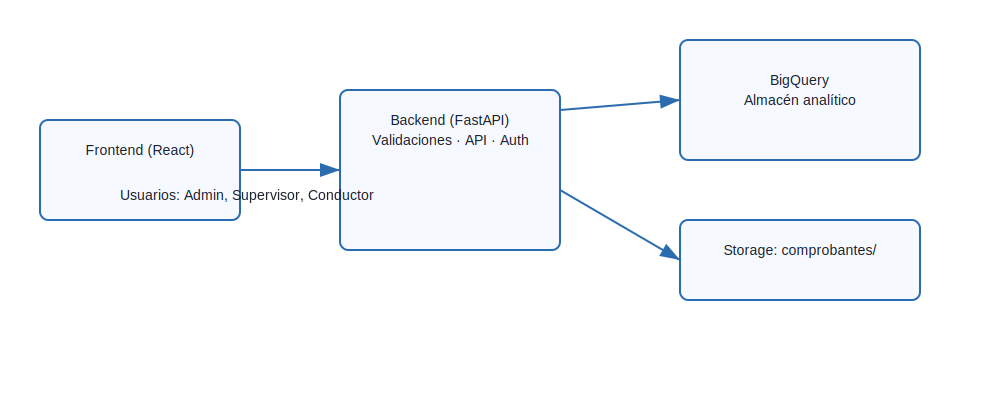
\includegraphics[width=0.9\textwidth]{Images/Project/architecture.pdf}
	\caption{Diagrama de arquitectura general del prototipo XCargo.}
	\label{fig:arquitectura}
\end{figure}

\noindent Referencias sobre frameworks y plataformas utilizados: FastAPI para la construcción de APIs y React para el frontend son soluciones ampliamente adoptadas por su rendimiento y ecosistema \cite{fastapi2020, react2013}.

\section{Modelo de datos y diseño de identificadores}
El diseño del modelo de datos prioriza la trazabilidad: cada registro de pago incluye un identificador de transacción (`Id_Transaccion`), referencia bancaría, fecha/hora, identificador del conductor y punteros a los comprobantes. Para evitar condiciones de carrera en la generación de `Id_Transaccion`, se describe una opción de mejora (uso de UUID o generación centralizada con control de concurrencia) que se evaluará en la fase de pruebas.

\section{Fuentes de datos}
Las fuentes de datos utilizadas durante el prototipo son:
\begin{itemize}
	\item Tablas BigQuery (p. ej. `pagosconductor`, `guias_liquidacion`, `COD_pendientes_v1`).
	\item Archivos de comprobantes almacenados en `backend/comprobantes/`.
	\item Datos de prueba sintetizados para simular escenarios de conciliación y duplicados.
\end{itemize}

\begin{figure}[htbp]
	\centering
	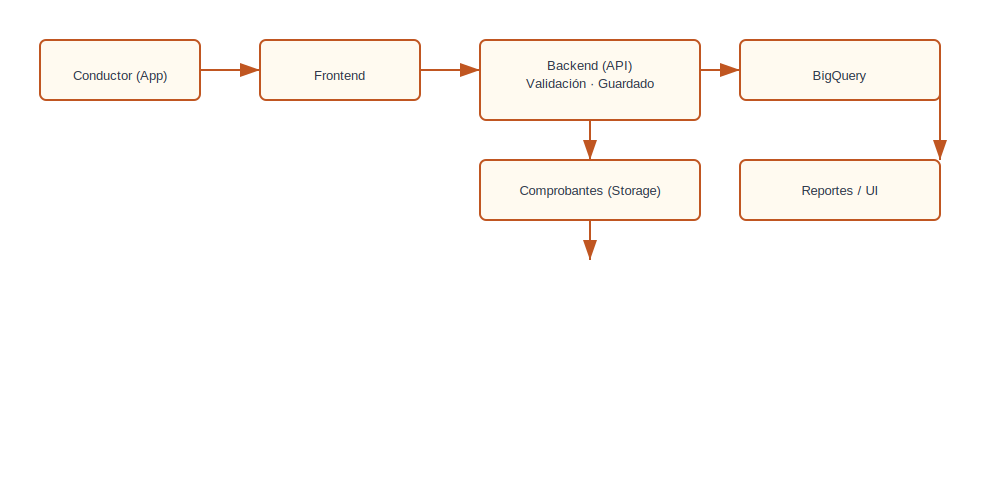
\includegraphics[width=0.85\textwidth]{Images/Project/dataflow.pdf}
	\caption{Flujo de datos: registro de pago, subida de comprobante y conciliación analítica.}
	\label{fig:dataflow}
\end{figure}

\noindent El uso de BigQuery como almacén analítico se documenta ampliamente en la literatura de plataformas en nube y se discuten consideraciones de latencia y coste \cite{bigquery2011}.

\section{Implementación}
La implementación sigue prácticas de desarrollo ágil en ciclos cortos: despliegues locales con `uvicorn --reload` para pruebas rápidas y conjunto de scripts para poblar BigQuery con datos de prueba. Se documentan los endpoints principales y las rutas de uso en el repositorio.

\section{Plan de pruebas y validación}
Las pruebas se estructuran en:
\begin{itemize}
	\item Pruebas unitarias: funciones de validación y utilidades en el backend.
	\item Pruebas de integración: secuencias completas (registro de pago con subida de comprobantes y verificación en BigQuery).
	\item Pruebas funcionales: escenarios reales y edge cases (referencias duplicadas, comprobantes faltantes, formatos incorrectos).
	\item Pruebas de rendimiento: consultas repetidas a BigQuery para estimar latencias y costos por consulta.
\end{itemize}

\section{Métricas de evaluación}
Se definen métricas cuantitativas para evaluar el impacto del prototipo:
\begin{itemize}
	\item Tiempo promedio de conciliación por transacción (antes y después del prototipo).
	\item Tasa de discrepancia (porcentaje de transacciones con errores o duplicados).
	\item Tasa de éxito de conciliación automática (porcentaje de transacciones conciliadas sin intervención manual).
	\item Latencia promedio de consultas analíticas en BigQuery y costo estimado por 1.000 consultas.
\end{itemize}

\section{Consideraciones éticas y de seguridad}
Se incluye el manejo responsable de datos personales (correos, identificadores) y la recomendación de cifrar secretos (mover `SECRET_KEY` a variables de entorno) y restringir el acceso a los comprobantes. En la evaluación se considerarán prácticas de anonimización si se trabaja con datos reales.

\section{Limitaciones}
Se reconocen limitaciones propias del prototipo: uso de almacenamiento local para comprobantes, ausencia de pasarela de pagos integrada y limitaciones de BigQuery como datastore transaccional. Estas restricciones se explican y se proponen líneas de mejora.

    
    % Capitulo 2
    \chapter{Cap\'{i}tulo 2}
    % Capítulo 2 - Implementación (Borrador)
\chapter{Implementación}

En este capítulo se documenta la implementación del prototipo XCargo. Se describen los componentes principales del backend y frontend, los endpoints disponibles, los modelos de datos usados en las comunicaciones y las responsabilidades de cada módulo.

\section{Resumen arquitectónico}
El sistema sigue una arquitectura cliente-servidor clásica:
\begin{itemize}
\item Frontend: aplicación React + TypeScript (Vite) que gestiona la autenticación, vistas según rol y la subida de comprobantes.
\item Backend: API REST implementada con FastAPI. Opera sobre tablas analíticas en Google BigQuery y un almacenamiento local de comprobantes (`backend/comprobantes/`) para el prototipo.
\item Almacenamiento analítico: BigQuery para consultas agregadas y conciliaciones.
\end{itemize}

\section{Endpoints principales}
A continuación se presenta una tabla resumen de los endpoints más relevantes (ruta, método y objetivo).

\begin{tabular}{p{5cm} p{2cm} p{8cm}}
Ruta & Método & Propósito \\
\hline
/auth/login & POST & Autenticación y emisión de JWT con rol y permisos \\
/auth/solicitar-codigo & POST & Solicitar código de recuperación de contraseña \\
/auth/cambiar-clave & POST & Cambiar contraseña con código de verificación \\
/guias/pendientes & GET & Obtener guías pendientes de liquidación para un conductor \\
/guias/sincronizar-guias-desde-cod & POST & Sincronizar guías desde la tabla COD_pendientes_v1 \\
/pagos/registrar-conductor & POST & Registrar pago de conductor, validar y guardar comprobantes \\
/pagos/ (otros) & POST/GET & Endpoints para pagos avanzados y conciliaciones \\
/conciliacion/ (varios) & GET/POST & Endpoints para procesos de conciliación y reportes \\
/roles/ & GET/POST & Gestión de roles y permisos \\
\end{tabular}

\subsection{Listado ampliado de endpoints}
Basado en la revisión del código, los routers disponibles incluyen (lista no exhaustiva):
\begin{itemize}
\item `/auth/*` — login, solicitar-codigo, cambiar-clave
\item `/guias/*` — pendientes, sincronizar-guias-desde-cod, operaciones de liquidación
\item `/pagos/*` — registrar-conductor, endpoints avanzados de pagos y validación
\item `/pagos-avanzados/*` — validar-pago, procesar-pago-completo
\item `/conciliacion/*` — carga de archivos bancarios, ejecución de conciliaciones por lote, auditoría y gestión de estados
\item `/cruces/*` — obtención de cruces bancarios, estadísticas y acciones manuales (aprobar/rechazar)
\item `/contabilidad/*` — resúmenes contables, reportes por cliente
\item `/admin/*` — gestión administrativa: crear usuarios, buscar usuarios, listar entregas
\item `/master/*` — dashboards globales y exportaciones para usuarios con rol master/admin
\item `/roles/*` — listado y gestión de roles
\item `/ocr/*` — extracción OCR con IA (extraer), health check
\item `/pago-cliente/*` — registrar pagos por cliente y enviar confirmaciones por email
\end{itemize}

\section{Ejemplos de uso: request/response}
Se muestran a continuación tres ejemplos representativos (resumidos) que pueden incluirse en la documentación técnica.

\subsection{Login (`/auth/login`)}
Request (JSON):
\begin{verbatim}
POST /auth/login
{
    "correo": "juan@xcargo.co",
    "password": "miContrasena"
}
\end{verbatim}

Response (JSON):
\begin{verbatim}
{
    "id_usuario": "USR_...",
    "nombre": "Juan",
    "correo": "juan@xcargo.co",
    "rol": "conductor",
    "permisos": [...],
    "token": "eyJhbGci..."
}
\end{verbatim}

\subsection{Registrar pago conductor (`/pagos/registrar-conductor`)}
Request (multipart/form-data): campos principales:
\begin{verbatim}
POST /pagos/registrar-conductor
Form fields:
    correo: conductor@xcargo.co
    valor_pago_str: 120000
    fecha_pago: 2025-07-02
    hora_pago: 14:03
    tipo: transferencia
    entidad: Bancolombia
    referencia: REF12345
    guias: [{"tracking":"TRK123","referencia":"REF_G1","valor":50000}]
Files:
    comprobante_0: archivo.jpg
    comprobante_1: archivo2.jpg (opcional)
\end{verbatim}

Response (JSON) (resumen):
\begin{verbatim}
{
    "status": "ok",
    "Id_Transaccion": 2345,
    "comprobantes": ["https://api.x-cargo.co/static/uuid_...jpg"],
    "detalle": "Pago registrado y pendiente de conciliación"
}
\end{verbatim}

\subsection{Ejecutar conciliación por lote (`/conciliacion/ejecutar-conciliacion-lote`)}
Request (JSON):
\begin{verbatim}
POST /conciliacion/ejecutar-conciliacion-lote
{
    "fecha_inicio": "2025-06-01",
    "fecha_fin": "2025-07-01",
    "estrategia": "por_valor"
}
\end{verbatim}

Response (JSON) (resumen):
\begin{verbatim}
{
    "procesadas": 1520,
    "conciliadas_exacto": 1200,
    "conciliadas_aproximado": 200,
    "pendientes": 120,
    "detalle_url": "/conciliacion/reportes/2025-10-14"
}
\end{verbatim}


Notas:
\begin{itemize}
\item Muchos endpoints utilizan BigQuery para validaciones en tiempo de escritura (por ejemplo verificación de referencias duplicadas, búsquedas por tracking).
\item La generación de `Id_Transaccion` actualmente se hace consultando `MAX(Id_Transaccion)` y sumando 1 por lote; se recomienda reemplazarlo por UUID o un generador centralizado para evitar condiciones de carrera.
\end{itemize}

\section{Modelos de datos (resumen)}
Los modelos pydantic y estructuras JSON usadas en las comunicaciones incluyen (resumen):
\begin{itemize}
\item `PagoRequest`: lista de facturas/guías, valor, fecha, banco, tipo, referencia y operador.
\item `GuiaAsignada` / `RegistroPago`: estructuras para asignar valor por guía dentro de una referencia de pago.
\item `Usuario` (implícito): datos devueltos por `auth/login` incluyen id_usuario, nombre, correo, rol, permisos y token JWT.
\end{itemize}

\section{Flujos principales}
\subsection{Registro de pago por conductor}
Flujo simplificado:
\begin{enumerate}
\item El conductor completa un formulario en el frontend y adjunta comprobantes.
\item El frontend envía un request multipart/form-data a `/pagos/registrar-conductor`.
\item El backend valida formato, referencia, fechas, y consulta BigQuery para obtener datos relacionados (p. ej. `COD_pendientes_v1`).
\item Si todo es válido, guarda comprobantes en `backend/comprobantes/` y persiste filas en `pagosconductor` en BigQuery con `Id_Transaccion` común por lote.
\item Se retorna un objeto con estado y URL(s) de comprobante(s).
\end{enumerate}

\subsection{Consulta de guías pendientes}
El endpoint `/guias/pendientes` obtiene guías de `guias_liquidacion` y `COD_pendientes_v1`, aplica filtros (estado 360, fechas, exclusión de pagadas) y devuelve una lista limpia priorizando `guias_liquidacion`.

\section{Frontend: responsabilidades y componentes}
El frontend está organizado con un `AuthContext` que maneja el token JWT y la lista de permisos. Componentes y responsabilidades clave:
\begin{itemize}
\item `ProtectedRoute`: protege rutas según permisos del usuario.
\item Formularios de registro de pago: envían multipart/form-data con campos y múltiples comprobantes (`comprobante_0`, `comprobante_1`, ...).
\item Páginas por rol: dashboards para administradores, supervisores, y vistas simplificadas para conductores.
\end{itemize}

\section{Consideraciones operativas y de seguridad}
\begin{itemize}
\item Mover `SECRET_KEY` fuera del código a variables de entorno o un secreto gestionado.
\item Validar límites y tipos de archivos para comprobantes (ya implementado con tamaños y extensiones permitidas).
\item Revisar concurrencia en generación de identificadores y operaciones que usan `MAX(...) + 1`.
\end{itemize}

\section{Ejemplos y snippets}
Ejemplo resumido (respuesta de login):
\begin{verbatim}
{
  "id_usuario": 123,
  "nombre": "Juan",
  "correo": "juan@xcargo.co",
  "rol": "conductor",
  "permisos": [...],
  "token": "eyJhbGci..."
}
\end{verbatim}

\section{Tareas pendientes para la implementación final}
\begin{itemize}
\item Añadir pruebas unitarias e integración para endpoints críticos (pagos, guías, auth).
\item Documentar contratos (request/response) más detalladamente y agregar ejemplos en el README técnico.
\item Considerar migrar comprobantes a almacenamiento en la nube (GCS) para producción.
\end{itemize}
Existen varias normas para la citaci\'{o}n bibliogr\'{a}fica. Algunas \'{a}reas del conocimiento prefieren normas espec\'{\i}ficas para citar las referencias bibliogr\'{a}ficas en el texto y escribir la lista de bibliograf\'{\i}a al final de los documentos. Esta plantilla brinda la libertad para que el autor de la tesis  o trabajo de investigaci\'{o}n utilice la norma bibliogr\'{a}fica com\'{u}n para su disciplina. Sin embargo, se solicita que la norma seleccionada se utilice con rigurosidad, sin olvidar referenciar "todos" los elementos tomados de otras fuentes (referencias bibliogr\'{a}ficas, patentes consultadas, software empleado en el manuscrito, en el tratamiento a los datos y resultados del trabajo, consultas a personas (expertos o p\'{u}blico general), entre otros).\\

\section{Ejemplos de citaciones bibliogr\'{a}ficas}

Citaci\'{o}n individual:\cite{AG01}.\\
Citaci\'{o}n simult\'{a}nea de varios autores:
\cite{AG12,AG52,AG70,AG08a,AG09a,AG36a,AG01i}.\\

Por lo general, las referencias bibliogr\'{a}ficas correspondientes a los anteriores n\'{u}meros, se listan al final del documento en orden de aparici\'{o}n o en orden alfab\'{e}tico. Otras normas de citaci\'{o}n incluyen el apellido del autor y el a\~{n}o de la referencia, por ejemplo: 1) "...\'{e}nfasis en elementos ligados al \'{a}mbito ingenieril que se enfocan en el manejo de datos e informaci\'{o}n estructurada y que seg\'{u}n Kostoff (1997) ha atra\'{\i}do la atenci\'{o}n de investigadores dado el advenimiento de TIC...", 2) "...Dicha afirmaci\'{o}n coincide con los planteamientos de Snarch (1998), citado por Castellanos (2007), quien comenta que el manejo..." y 3) "...el futuro del sistema para argumentar los procesos de toma de decisiones y el desarrollo de ideas innovadoras (Nosella \textsl{et al}., 2008)...".\\

\section{Ejemplos de presentaci\'{o}n y citaci\'{o}n de figuras}
Las ilustraciones forman parte del contenido de los cap\'{\i}tulos. Se deben colocar en la misma p\'{a}gina en que se mencionan o en la siguiente (deben siempre mencionarse en el texto).\\

Las llamadas para explicar alg\'{u}n aspecto de la informaci\'{o}n deben hacerse con nota al pie y su nota correspondiente\footnote{Las notas van como "notas al pie". Se utilizan para explicar, comentar o hacer referencia al texto de un documento, as\'{\i} como para introducir comentarios detallados y en ocasiones para citar fuentes de informaci\'{o}n (aunque para esta opci\'{o}n es mejor seguir en detalle las normas de citaci\'{o}n bibliogr\'{a}fica seleccionadas).}. La fuente documental se debe escribir al final de la ilustraci\'{o}n o figura con los elementos de la referencia (de acuerdo con las normas seleccionadas) y no como pie de p\'{a}gina. Un ejemplo para la presentaci\'{o}n y citaci\'{o}n de figuras, se presenta a continuaci\'{o}n (citaci\'{o}n directa):\\

Por medio de las propiedades del fruto, seg\'{u}n el espesor del endocarpio, se hace una clasificaci\'{o}n de la palma de aceite en tres tipos: Dura, Ternera y Pisifera, que se ilustran en la Figura
\ref{fig:yoda2}.\\
\begin{figure}
    \centering%
    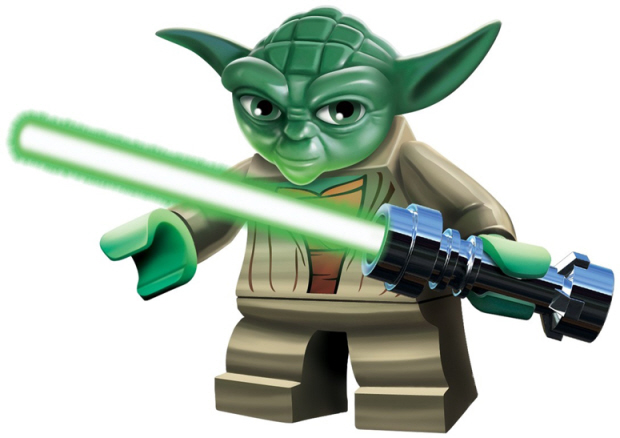
\includegraphics{Images/ImagenYoda.jpg}%
    \caption{Lego StarWars~\cite{LucasArts2010Yoda} }
    \label{fig:yoda2}
\end{figure}

\section{Ejemplo de presentaci\'{o}n y citaci\'{o}n de tablas y cuadros}
Para la edici\'{o}n de tablas, cada columna debe llevar su t\'{\i}tulo; la primera palabra se debe escribir con may\'{u}scula inicial y preferiblemente sin abreviaturas. En las tablas y cuadros, los t\'{\i}tulos y datos se deben ubicar entre l\'{\i}neas horizontales y verticales cerradas (como se realiza en esta plantilla).\\

La numeraci\'{o}n de las tablas se realiza de la misma manera que las figuras o ilustraciones, a lo largo de todo el texto. Deben llevar un t\'{\i}tulo breve, que concreta el contenido de la tabla; \'{e}ste se debe escribir en la parte superior de la misma. Para la presentaci\'{o}n de cuadros, se deben seguir las indicaciones dadas para las tablas.\\

Un ejemplo para la presentaci\'{o}n y citaci\'{o}n de tablas (citaci\'{o}n indirecta), se presenta a continuaci\'{o}n:\\

De esta participaci\'{o}n aproximadamente el 60 \% proviene de biomasa
(Tabla \ref{EMundo1}).
\begin{center}
\begin{threeparttable}
    \centering%
    \caption{Participaci\'{o}n de las energ\'{\i}as renovables en el suministro total de energ\'{\i}a primaria \cite{AG02i}.}
    \label{EMundo1}
    \begin{tabular}{|l|c|c|}
        \hline
        & \multicolumn{2}{c|}{Participaci\'{o}n en el suministro de energ\'{\i}a primaria /\% (Mtoe)\;$\tnote{1}$}\\
        \cline{2-3}%
        {Region} & Energ\'{\i}as renovables & Participaci\'{o}n de la biomasa\\
        \hline%
        Latinoam\'{e}rica&28,9 (140)&62,4 (87,4)\\
        \hline%
        \:Colombia&27,7 (7,6)&54,4 (4,1)\\
        \hline%
        Alemania&3,8 (13,2)&65,8 (8,7)\\
        \hline%
        Mundial&13,1 (1404,0)&79,4 (1114,8)\\
        \hline
    \end{tabular}
    \begin{tablenotes}
        \item[1] \footnotesize{1 kg oe=10000 kcal=41,868 MJ}
    \end{tablenotes}
\end{threeparttable}
\end{center}

NOTA: en el caso en que el contenido de la tabla o cuadro sea muy extenso, se puede cambiar el tama\~{n}o de la letra, siempre y cuando \'{e}sta sea visible por el lector.\\

\subsection{Consideraciones adicionales para el manejo de figuras y tablas}
Cuando una tabla, cuadro o figura ocupa m\'{a}s de una p\'{a}gina, se debe repetir su identificaci\'{o}n num\'{e}rica, seguida por la palabra continuaci\'{o}n.\\

Adicionalmente los encabezados de las columnas se deben repetir en todas las p\'{a}ginas despu\'{e}s de la primera.\\

Los anteriores lineamientos se contemplan en la presente plantilla.\\

\begin{itemize}
\item Presentaci\'{o}n y citaci\'{o}n de ecuaciones.
\end{itemize}

La citaci\'{o}n de ecuaciones, en caso que se presenten, debe hacerse como lo sugiere esta plantilla. Todas las ecuaciones deben estar numeradas y citadas detro del texto.\\

Para el manejo de cifras se debe seleccionar la norma seg\'{u}n el \'{a}rea de conocimiento de la tesis  o trabajo de investigaci\'{o}n.\\
    
    % Capitulo 3
    \chapter{Cap\'{i}tulo 3}
    Se deben incluir tantos cap\'{\i}tulos como se requieran; sin embargo, se recomienda que la tesis  o trabajo de investigaci\'{o}n tenga un m\'{\i}nimo 3 cap\'{\i}tulos y m\'{a}ximo de 6 cap\'{\i}tulos (incluyendo las conclusiones).\\
    
    % Capitulo 4
    \chapter{Cap\'{i}tulo 4}
    Se deben incluir tantos cap\'{\i}tulos como se requieran; sin embargo, se recomienda que la tesis  o trabajo de investigaci\'{o}n tenga un m\'{\i}nimo 3 cap\'{\i}tulos y m\'{a}ximo de 6 cap\'{\i}tulos (incluyendo las conclusiones).\\
    
    % Capitulo 5
    \chapter{Cap\'{i}tulo 5}
    Se deben incluir tantos cap\'{\i}tulos como se requieran; sin embargo, se recomienda que la tesis  o trabajo de investigaci\'{o}n tenga un m\'{\i}nimo 3 cap\'{\i}tulos y m\'{a}ximo de 6 cap\'{\i}tulos (incluyendo las conclusiones).\\

    
    % Capitulo 10
    \chapter{Conclusiones y recomendaciones}
    \section{Conclusiones}
Las conclusiones constituyen un cap\'{\i}tulo independiente y presentan, en forma l\'{o}gica, los resultados de la tesis  o trabajo de investigaci\'{o}n. Las conclusiones deben ser la respuesta a los objetivos o prop\'{o}sitos planteados. Se deben titular con la palabra conclusiones en el mismo formato de los t\'{\i}tulos de los cap\'{\i}tulos anteriores (T\'{\i}tulos primer nivel), precedida por el numeral correspondiente (seg\'{u}n la presente plantilla).\\

\section{Recomendaciones}
Se presentan como una serie de aspectos que se podr\'{\i}an realizar en un futuro para emprender investigaciones similares o fortalecer la investigaci\'{o}n realizada. Deben contemplar las perspectivas de la investigaci\'{o}n, las cuales son sugerencias, proyecciones o alternativas que se presentan para modificar, cambiar o incidir sobre una situaci\'{o}n espec\'{\i}fica o una problem\'{a}tica encontrada. Pueden presentarse como un texto con caracter\'{\i}sticas argumentativas, resultado de una reflexi\'{o}n acerca de la tesis o trabajo de investigaci\'{o}n.\\
    
    
    % Anexos (Opcional)
    % \chapter*{Anexos}
    % % \section{Manual de instalación}

% \section{Manual de usuario}

% \section{Informe de ejecución de pruebas}


    
    % Indices (Opcional)
    % \chapter*{\'Indices}
    % \input{BackMatter/B10-Index}
    
    % Incluye las referencias
    %\bibliographystyle{apalike}
    \bibliographystyle{unsrt}
    \bibliography{Bibliography/referencias}

\end{document}
